\documentclass[a4paper, 11pt, openleft]{memoir}

\usepackage{indentfirst}

% Fonts
\usepackage[no-math]{fontspec}
\setmainfont{ZillaSlab}[
    Path = fonts/,
    Extension = .ttf,
    UprightFont = *-Regular,
    ItalicFont = *-Italic,
    BoldFont = *-Bold,
    BoldItalicFont = *-BoldItalic,
    Ligatures = {TeX, Common}
]
% \setmainfont{IosevkaCustom}[
%     Path = fonts/,
%     Extension = .ttf,
%     UprightFont = *-CondensedLight,
%     ItalicFont = *-CondensedLightItalic,
%     BoldFont = *-CondensedHeavy,
%     BoldItalicFont = *-CondensedHeavyItalic,
%     Ligatures = {TeX, Common},
%     Scale = 0.9
% ]
\setmonofont[Scale = MatchLowercase]{IosevkaCustom}[
    Path = fonts/,
    Extension = .ttf,
    UprightFont = *-CondensedMedium,
    ItalicFont = *-CondensedMediumItalic,
    BoldFont = *-CondensedHeavy,
    BoldItalicFont = *-CondensedHeavyItalic,
    Ligatures = {TeX, Common},
    Scale = 0.9
]
\defaultfontfeatures{Mapping = tex-text, Scale = MatchLowercase}
\usepackage{mathtools}
\usepackage[math-style = TeX, mathrm = sym, warnings-off = {mathtools-colon}]{unicode-math}
\setmathfont[Scale = MatchLowercase]{Concrete-Math.otf}
\setoperatorfont\symscr
\newcolumntype{C}{>{$}c<{$}}
\newcolumntype{L}{>{$}l<{$}}
\newcolumntype{R}{>{$}r<{$}}

% Page Layout and Margins
\setsecnumdepth{subsection}
\settocdepth{subsection}
\setlrmarginsandblock{4cm}{1cm}{*}
\setulmarginsandblock{3cm}{2cm}{*}
\setlength{\headheight}{30pt}
\addtolength{\topmargin}{-10pt}
\setlength{\parindent}{1.5cm}
\setlength{\parskip}{0.3em}
\setlength{\beforechapskip}{20pt}
\noDisplayskipStretch
\allowdisplaybreaks
\setSpacing{1.4}
\XeTeXlinebreakskip=0pt plus 3pt
\checkandfixthelayout

% Footnotes
\usepackage{fancyhdr}
\pagestyle{fancy}
\fancyhead[LE]{\textbf{\thepage ~ $\big\vert$ \leftmark ~(Revision: \today, Puripat Thumbanthu)}}
\fancyhead[RO]{\textbf{(Revision: \today, Puripat Thumbanthu) ~\rightmark ~ $\big\vert$ \thepage}}
\fancyhead[RE, LO, C]{}

% Indices
\usepackage{imakeidx}
\makeindex

% Packages
\usepackage[dvipsnames]{xcolor}
\usepackage{caption, subcaption, graphicx, pdfpages, float, wrapfig}
\usepackage[inkscapeversion = 1, inkscapelatex = true]{svg}
\svgpath{{diagrams/}}
\graphicspath{{diagrams/}}
\usepackage[inline]{enumitem}
\usepackage{multicol}
\setlength{\columnseprule}{1pt}
\def\columnseprulecolor{\color{lightgray}}
\usepackage{minted}
\setminted{
    frame = lines,
    bgcolor = lightgray,
    linenos,
    breaklines,
    style = algol_nu
}

\usepackage{csquotes}

% Styling Figures
\DeclareCaptionLabelSeparator{pipe}{ $\vert$ }
\captionsetup{
    labelfont = {bf},
    font = {small, sc},
    width = 0.6\textwidth,
    labelsep = pipe,
    figurename = \textbf{Fig. }
}

% Styling Titles
\renewcommand{\partnamefont}{\LARGE\bfseries\scshape\centering}
\renewcommand{\partnumfont}{\LARGE\bfseries\scshape\centering\MakeUppercase}
\renewcommand{\midpartskip}{\par\rule{1in}{0.5pt}\vspace{1em}\par}
\renewcommand{\printparttitle}{\HUGE\bfseries\scshape\centering}
\renewcommand{\afterpartskip}{\relax}
\chapterstyle{veelo}
    \renewcommand*{\printchapternum}{%
    \makebox[0pt][l]{%
    \hspace{.8em}%
    \resizebox{!}{\beforechapskip}%
    {\chapnumfont \thechapter}%
    \hspace{.8em}%
    \rule{2\midchapskip}{\beforechapskip}%
    }%
}

% Hyperlinks
\usepackage[colorlinks, linkcolor = blue]{hyperref}
\usepackage{cleveref}

% Definition/Theorems, and Examples
\usepackage{tcolorbox}
\tcbuselibrary{theorems, breakable}
\newtcbtheorem[auto counter, crefname = {theorem}{theorems}, Crefname = {Theroem}{Theorems}]{thm}{Theorem}{
    sharp corners, colback = lightgray!40, breakable
}{thm}
\newtcbtheorem[auto counter, crefname = {axiom}{axioms}, Crefname = {Axiom}{Axioms}]{axiom}{Axiom}{
    sharp corners, colback = lightgray!40, breakable
}{axiom}
\newtcbtheorem[auto counter, crefname = {definition}{definition}, Crefname = {Definition}{Definition}]{df}{Definition}{
    sharp corners, colback = lightgray!40, colframe = darkgray, breakable
}{df}
\newtcbtheorem[auto counter, crefname = {lemma}{lemma}, Crefname = {Lemma}{Lemma}]{lemma}{Lemma}{
    sharp corners,
}{lemma}
\newtcbtheorem[auto counter, number within = section]{exmp}{Example}{
    colback = lightgray!40, colframe = darkgray, breakable
}{exmp}
\newtcbtheorem[auto counter, number within = chapter, crefname = {remarks of chapter }{remarks of chapter }, Crefname = {Remarks}{Remarks}]{remark}{Remarks on chapter }{
    colback = lightgray!10, colframe = black, breakable
}{remark}
% Proofs
\usepackage{amsthm}

% Conclusions
\newcommand{\conclusion}{\section{Conclusion for Chapter \thechapter}}
\newcommand{\formula}{\section{Formula from Chapter \thechapter}}
\newcommand{\prelude}[1]{
    \chapter*{Prelude: #1}
    \addcontentsline{toc}{chapter}{Prelude: #1}
}
\newcommand{\chapterexercises}{\section{Exercises for Chapter \thechapter}}

%%% Notation Commands

\usepackage[]{siunitx}
\usepackage{physics}
\AtBeginDocument{\RenewCommandCopy\qty\SI}

% Geometry
\let\line\overline
% Mathematical constants
\newcommand{\e}{\symrm{e}}
\newcommand{\im}{\symrm{i}}
\newcommand{\cpi}{\symrm{\pi}}
\DeclareMathOperator*{\ssum}{\symrm{\Sigma}}
\DeclareMathOperator*{\Proj}{\symrm{Proj}}
\DeclareMathOperator*{\fgamma}{\symrm{\Gamma}}
% Vector notations
\newcommand{\vv}[1]{\pmb{\symrm{#1}}}
\newcommand{\conj}{^{\ast}}
\newcommand{\dagr}{^{\dag}}
\newcommand{\trnsp}{^{\intercal}}
\newcommand{\iden}{\symbb{I}}
\renewcommand\vdot\cdot
% e Unit vectors
\newcommand{\uv}[1]{\hat{\vv{e}}_{#1}}
% Kronecker delta and Dirac's delta function
\newcommand{\kdel}[1]{\symrm{\delta}_{#1}}
\newcommand{\ddel}{\symrm{\delta}}
% Discrete differences
\newcommand{\Dd}[1]{\symrm{\Delta}{#1}}
% Limit arrows
\newcommand{\appr}{\rightarrow}
% Physics quantities symbols
\newcommand{\lagr}{\mathcal{L}}
\newcommand{\haml}{\mathcal{H}}
\newcommand{\hilb}{\mathcal{E}}
% Path integral measures
\newcommand{\pintm}[1]{\mathcal{D}[#1]}
% Density matrix
\newcommand{\dnst}{\hat{\rho}}

% Unit vectors i j k
\newcommand{\ihat}{\hat{\i}}
\newcommand{\jhat}{\hat{\j}}
\newcommand{\khat}{\hat{k}}
% Tensor products
\newcommand{\tensor}{\otimes}
% And, and or, in math expressions
\newcommand{\mathand}{\quad\textrm{and,}\quad}
\newcommand{\mathor}{\quad\textrm{or,}\quad}

% Set theory notations
\NewDocumentCommand{\comp}{}{^\complement}

\newcommand{\prerequisites}[1]{\textbf{Prerequisites:}~\emph{#1}}

% Bibliographies
\usepackage[
    backend = biber,
    style = phys,
    sorting = anyvt
]{biblatex}
\addbibresource{bibliography.bib}

% TikZ
\usepackage{tikz, pgfplots, tikz-3dplot}
\pgfplotsset{compat = 1.18}

\usetikzlibrary{external}
\tikzexternalize[prefix = tikz/]

\usetikzlibrary{calc}
\usetikzlibrary{angles, quotes}
\usetikzlibrary{patterns}
\usetikzlibrary{decorations.pathreplacing, calligraphy}
\usetikzlibrary{3d}

\tikzstyle{brace} = [decorate, decoration = {brace, amplitude = 5pt, raise = 2pt}]
\tikzstyle{mirrored brace} = [decorate, decoration = {brace, amplitude = 3pt, raise = 2pt, mirror}]
\tikzstyle{unit} = [ultra thick, blue, -stealth]
\tikzstyle{axis} = [thick, -stealth]
\tikzstyle{vector} = [-latex]
\tikzstyle{line} = [latex-latex]

\usepackage[symbols, nogroupskip]{glossaries-extra}
\setabbreviationstyle[acronym]{long-short}

\newglossarystyle{longright}{%
    \setglossarystyle{long}%
    \renewenvironment{theglossary}{%
        \renewcommand{\arraystretch}{1.1} % Adjust the line spacing here
        \begin{longtable}{@{}p{0.25\linewidth}p{0.75\linewidth}}}%
        {\end{longtable}}%
    \renewcommand{\glossentry}[2]{%
        \glsentryitem{##1}\glstarget{##1}{\glossentryname{##1}} &
        \raggedleft\glossentrydesc{##1}\tabularnewline
    }%
    \renewcommand*{\glsgroupskip}{}
}

\makeglossaries

\glsxtrnewsymbol[description = {Identity unit}]{unit}{$\mathbb{1}$}
\glsxtrnewsymbol[description = {Extension of arbritary operator $A$ defined in $\hilb_n$ onto $\hilb$}]{operatorextension}{$\tilde{A}$}
\glsxtrnewsymbol[description = {Path integral measure on a variable}]{pintm}{$\pintm{q}$}
\glsxtrnewsymbol[description = {The Euler's constant}]{e}{$\e$}
\glsxtrnewsymbol[description = {Hilbert space of the whole system}]{hilb}{$\hilb$}
\glsxtrnewsymbol[description = {The $n$\textsuperscript{th} subspace of Hilbert space}]{hilbsub}{$\hilb_n$}
\glsxtrnewsymbol[description = {Planck's constant}]{planck}{$h$}
\glsxtrnewsymbol[description = {Reduced Planck's constant. $\hbar = {h}/{2\cpi}$}]{reducedplanck}{$\hbar$}
\glsxtrnewsymbol[description = {Hamiltonian of a system}]{haml}{$\haml$}
\glsxtrnewsymbol[description = {The imaginary unit}]{i}{$\im$}
\glsxtrnewsymbol[description = {The identity matrix/identity operator}]{iden}{$\iden$}
\glsxtrnewsymbol[description = {Propagator from point $q_F, t_F$ to $q_0, t_0$ using the Lagrangian of particle $\mathcal{A}$}]{propagator}{$K_{\mathcal{A}}(q_F, t_F; q_0, t_0)$}
\glsxtrnewsymbol[description = {Propagator of a separable system. Extra arguments represents the usage on bipartite systems.}]{propagatorseparable}{$K_0(q\prime, t\prime; q_0, t_0)$}
\glsxtrnewsymbol[description = {Generalized momentum}]{generalizedmomenetum}{$p$}
\glsxtrnewsymbol[description = {Generalized position}]{generalizedposition}{$q$}
\glsxtrnewsymbol[description = {Set of arbitrary basis $\ket{u_1}, \ket{u_2},\dots$ of a Hilbert space with index $i$}]{basis}{$\{\ket{u_i}\}$}
\glsxtrnewsymbol[description = {Time evolution operator. Evolves the time of the system from $t_A$ to $t_B$}]{timeevolve}{$\hat{U}(t_B, t_A)$}
\glsxtrnewsymbol[description = {Eigenvalue of arbritary ket $\ket{\psi}$}]{eigenvalue}{$\alpha_{\psi}$}
\glsxtrnewsymbol[description = {Ket of the whole system. Used when describing a bipartite system}]{ketofsystem}{$\ket{\eta}$}
\glsxtrnewsymbol[description = {Ket of the subsystems. Used when describing a monopartite system}]{ketofsystem2}{$\ket{\xi}$}
\glsxtrnewsymbol[description = {The Archimedes' constant}]{pi}{$\cpi$}
\glsxtrnewsymbol[description = {Tensor product}]{tenspr}{$\tensor$}

\makeatletter
\renewcommand*{\@@glossarysec}{section}
\makeatother

\begin{document}

\title{The study of the dynamics of quantum bipartite entangled systems using Feynman path integrals}
\author{Puripat Thumbanthu \\ Advisor: Assoc. Prof. Ekapong Hirunsirisawat, Dr. Tanapat Deesuwan}
\date{Started: May 16 2024}

\maketitle

\begin{center}
\emph{This version is not to be published. It is my own notes during the research.}
\end{center}

\tableofcontents*

\chapter{Introduction}

\section[Historical backgrounds]{Historical backgrounds\footnote{This introduction is rewritten after the school project has passed. I've declared this project to be independent of the school ever since. So, it's going to be much more authentic and straightforward.}}

Light, the first gateway to the quantum world of the humankind. I've always been intrigued by it. And, we've been able to confirm that light can be entangled, causing correlations in its polarization axes. Most modern development of physics has been into that field. But often, we tend to forget what we left behind four hundred years ago: the principle of least action. What happens when light passes through different medium? Refraction, everyone can answer that. But what happens if light is entangled?

To resolve this problem, I originally turned to the Schr\"odinger's equation for two particles. However, it's quite complex, and the mathematics behind it doesn't really elude me that much. So, I turned to the path integrals method. Its ability to intuitively produce the classical world, governed by the principle of least action, is captivating. The action principle appears so naturally in path integrals that I thought I was hallucinating. Question arises: what does the principle of least action looks like for a many body systems? Is it any different if they're entangled? I was literally mashing random words together at that point, but it has led me into the realm of physics that I don't think anyone really cares before: the dynamics of an entangled system.

Entanglement is usually defined as the inseparability of states, commonly used to describe the spin of a particle, which has been studied in great extent. It has found its use in quantum computer, giving its blazing speed. However, from my knowledge, no literatures has mentioned the effect of entanglement on the movement of particles. Will entangled particle move together in the same direction? If I separate a pair of entangled particles, put one in a potential, and let the other be free, does the particle in the potential have any effect on the free particle? And thus, this research (\emph{project}) was born.

This research started out by two people; me, and the other one that shall not be named. However, I have a lot of conflicts with that person. Long story short, he quitted; and thus, I'm on my own journey.

\printunsrtglossary[type = symbols, style = longright, title = {List of Symbols (Still incomplete)}]
\chapter{Generalization of the Gaussian integrals}

\section{Preliminary form}

A Gaussian integral is the integral of the Gaussian function $\exp[-x^2]$:
\begin{equation}
    \int_{\infty}^{-\infty} \exp[-x^2]\dd{x} = \sqrt{\cpi}.
\end{equation}
However, this is not that useful for path integrals, because it demands a more generalized form of this Gaussian function. Therefore, we focus on integrals of the form
\begin{equation}
    I_1 = \int_{\infty}^{-\infty} x^n\exp[-(ax^2 + bx + c)]\dd{x},\label{eq:generalized_gaussian}
\end{equation}
where $a$, $b$, and $c$ are constants and $n$ is a positive integer. This integral will be very useful later on when evaluating the Born expansion of the propagator.

Because we're just going to be dealing with integrals from negative to positive infinity, I shall omit the bounds of the integrals. Thus, every integral written with no bounds from now on are assumed to be a definite integral from negative to positive infinity.

\section{Evaluation}

To evaluate $I_1$ (\cref{eq:generalized_gaussian}), we shall complete the square first, then substitute the exponents to fit the form of the standard Gaussian integral.
\begin{align*}
    \int x^n\e^{-(ax^2 + bx + c)}\dd{x} &= \int x^n\exp[-a\left(x + \frac{b^2}{2a}\right)^2 + \frac{b^2}{4a} - c]\dd{x} \\
    &= \e^{\frac{b^2}{4a} - c}\int x^n\exp[-a\left(x + \frac{b^2}{2a}\right)]\dd{x}.
\end{align*}
Let
\begin{align}
    -u^2 &= -a\left(x + \frac{b^2}{2a}\right)^2 \\
    x &= \frac{u}{\sqrt{a}} - \frac{b^2}{2a} \\
    \dv{x}{u} &= \dv{u}(\frac{u}{\sqrt{a}} - \frac{b^2}{2a}) \\
    \dd{x} &= \frac{1}{\sqrt{a}}\dd{u}.
\end{align}
Then,
\begin{align}
    I_1 &= \e^{\frac{b^2}{4a} - c}\frac{1}{\sqrt{a}}\int\left(\frac{u}{\sqrt{a}} - \frac{b^2}{2a}\right)^n\e^{-u^2}\dd{u}. \\
    &= \e^{\frac{b^2}{4a} - c}\frac{1}{\sqrt{a}}\int\sum_{k = 0}^{n}{n \choose k}\left(\frac{b^2}{2a}\right)^{n - k}\left(\frac{u}{\sqrt{a}}\right)^k\e^{-u^2}\dd{u}. \\
    &= \e^{\frac{b^2}{4a} - c}\frac{1}{\sqrt{a}}\sum_{k = 0}^{n}\left[{n \choose k}\left(\frac{b^2}{2a}\right)^{n - k}\left(\frac{1}{\sqrt{a}}\right)^{k} \int u^k\e^{u^2}\dd{u}\right], \label{eq:generalized_gaussian-1}
\end{align}
i.e., $I_1$ can be written as a sum of
\begin{equation}
    I_0 = \int u^k\e^{-u^2}\dd{u}.
\end{equation}
Notice that when $n$ is odd, the integrand of $I_0$ is an odd function. Therefore, $I_0$ is zero whenever $n$ is odd. When $n$ is even however, the integrand is even. Thus, it can be simplified to
\begin{equation}
    2\int_{0}^{\infty} u^{2m}\e^{-u^2}\dd{u}
\end{equation}
where $k = 2m$. We then do another substitution by letting $-t = -u^2$. Thus, $u = \sqrt{t}$ and $\dd{u} = \flatfrac{\dd{t}}{2\sqrt{t}}$. Both infinity and zero aren't affected by a square root, therefore the bound doesn't change. Our integral then becomes
\begin{align}
    &2 \times \int_{0}^{\infty}t^{m}\e^{-t}\frac{1}{2\sqrt{t}}\dd{t}. \\
    &= \int_{0}^{\infty}t^{m - \frac{1}{2}}\e^{-t}\dd{t} \\
    &= \int_{0}^{\infty}t^{m + \frac{1}{2} - 1}\e^{-t}\dd{t} \\
    &= \fgamma\left(m + \frac{1}{2}\right) \\
    &= \fgamma\left(\frac{k + 1}{2}\right).
\end{align}
Since the integral evaluates to the gamma function for only even numbers, we add a term that makes $I_0 = 0$ when $n$ is odd:
\begin{equation}
    I_0 = \frac{1}{2}((-1)^k + 1)\fgamma\left(\frac{k + 1}{2}\right).
\end{equation}
Thus, from \cref{eq:generalized_gaussian-1},
\begin{equation}
    I_1 = \e^{\frac{b^2}{4a} - c}\frac{1}{\sqrt{a}}\sum_{k = 0}^{n}\left[{n \choose k}\left(\frac{b^2}{2a}\right)^{n - k}\left(\frac{1}{\sqrt{a}}\right)^{k} \frac{1}{2}((-1)^k + 1)\fgamma\left(\frac{k + 1}{2}\right)\right]
\end{equation}
To continue this, we then expand the combinatorics and use the formulas of arguments with half-integer real part to get
\begin{align}
    &\begin{multlined}
    \e^{\frac{b^2}{4a} - c}\frac{1}{\sqrt{a}}\sum_{k = 0}^{n}\frac{n!}{k!(n - k)!}\left(\frac{b^2}{2a}\right)^n\left(\frac{2a}{b^2}\right)^k\left(\frac{1}{\sqrt{a}}\right)^k\left(\sqrt{\cpi}\frac{k!}{4^{\frac{k}{2}}\left(\flatfrac{k}{2}\right)!}\right) \\
    \times \frac{1}{2}((-1)^k + 1)
    \end{multlined} \\
    &= \e^{\frac{b^2}{4a} - c}n!\sqrt{\frac{\cpi}{a}}\left(\frac{b^2}{2a}\right)^n\sum_{k = 0}^n\frac{1}{(n - k)!(\flatfrac{k}{2})!}\left(\frac{\sqrt{a}}{b^2}\right)^{k}\frac{1}{2}((-1)^k + 1)
\end{align}
To simplify the summation, we replace $k$ with $2k$, and the upper limit with $m$ where $m = \left\lfloor\flatfrac{n}{2}\right\rfloor$. Thus, we get
\begin{equation}
    \left[\sum_{k = 0}^{m}\frac{1}{(n - 2k)!k!}\left(\frac{\sqrt{a}}{b^2}\right)^{2k}\right]\e^{\frac{b^2}{4a} - c}n!\left(\frac{b^2}{2a}\right)^n\sqrt{\frac{\cpi}{a}}
\end{equation}
As far as I know, this equation cannot be simplified further.

\paragraph{Comment on the generalized Gaussian integral} Note that the integral in \cref{eq:generalized_gaussian} can be casted in the form of Meijer's $G$ function for $n \geq 0$:
\begin{multline}
    \int x^n\exp[-ax^2 - bx - c]\dd{x} \\= \frac{e^{-c}}{2\sqrt{\cpi}ab}\left[- \frac{2^{n + 1}a}{b^n} {G_{2, 1}^{1, 2}\left(\begin{matrix} \frac{1 - n}{2}, - \frac{n}{2}  \\0 \end{matrix} \middle| {\frac{4 a e^{- 2 i \pi}}{b^{2}}} \right)} + a^{\frac{1 - n}{2}}b {G_{1, 2}^{2, 1}\left(\begin{matrix} \frac{1 - n}{2}\\0, \frac{1}{2}\end{matrix} \middle| {\frac{b^{2}}{4 a}} \right)}\right]
\end{multline}
However, this form doesn't seem to be very helpful when we try to evaluate the polynomial part of the Gaussian integral because of the nature of the Meijer's $G$ function that's defined with integral of products.

\section{Tables of Gaussian integrals with varying orders}
\label{sec:table_of_gaussian_integrals}

\everymath{\displaystyle}
\begin{enumerate}[label = {$n = \arabic*$:}]
    \setcounter{enumi}{-1}
    \item $+\frac{1}{1}\sqrt{\frac{\cpi}{a}}\e^{\frac{b^2}{4a} - c}$
    \item $-\frac{b}{2}\sqrt{\frac{\cpi}{a^3}} \e^{\frac{b^2}{4a} - c}$
    \item $+\frac{1}{4}\sqrt{\frac{\cpi}{a^5}} (2a + b^2) \e^{\frac{b^2}{4a} - c}$
    \item $-\frac{b}{8}\sqrt{\frac{\cpi}{a^7}} (6a + b^2) \e^{\frac{b^2}{4a} - c}$
    \item $+\frac{1}{16}\sqrt{\frac{\cpi}{a^9}} (12a^2 + 12ab^2 + b^4)\e^{\frac{b^2}{4a} - c}$
    \item $-\frac{b}{32}\sqrt{\frac{\cpi}{a^{11}}} (60a^2 + 20ab^2 + b^2)\e^{\frac{b^2}{4a} - c}$
    \item $+\frac{1}{64}\sqrt{\frac{\cpi}{a^{13}}} (120a^3 + 180a^2b^2 + 30ab^4 + b^6)\e^{\frac{b^2}{4a} - c}$
    \item $-\frac{b}{128}\sqrt{\frac{\cpi}{a^{15}}} (840a^3 + 420a^2b^2 + 42ab^4 + b^6)\e^{\frac{b^2}{4a} - c}$
    \item $+\frac{1}{256}\sqrt{\frac{\cpi}{a^{17}}} (1680a^4 + 3360a^3b^2 + 840a^2b^4 + 56ab^6 + b^8)\e^{\frac{b^2}{4a} - c}$
    \item $-\frac{b}{512}\sqrt{\frac{\cpi}{a^{19}}} (15120a^4 + 10080a^3b^2 + 1512a^2b^4 + 72ab^6 + b^8)\e^{\frac{b^2}{4a} - c}$
\end{enumerate}
\chapter{Propagator and joint probability distribution in the position basis}

\section{General theory for the propagator of two particles}

\subsection{Non-interacting systems}

The propagator for a single particle system is used to find the probability distribution $\tilde{P}(x)$ of a state at anytime, i.e., for a state $\ket{\psi(t_0)}$ of a single particle,
\begin{equation}
    \tilde{P}(q_F, t_F) = \braket{q_F}{\psi(t_F)} = \int K(q_F, q_0; \Dd{t})\psi(q_0, t_0)\dd{q_0}.
\end{equation}
The probability of finding the particle at any point $(q_F, t_F)$ in spacetime is defined as
\begin{equation}
    P(q_F, t_F) \equiv |\tilde{P}(q_F, t_F)|^2
\end{equation}
This idea can be easily extended to describe any multiparticle system. But we shall only concern two particles systems in this study. Because the conventional notation is quite cumbersome, I shall introduce my own concise notation. From now on, every unprimed variable belong to particle one, and every unprimed variable, to particle one. E.g., the first particle Hilbert space shall be written with $\hilb$, and for the second particle, $\hilb_2$. This extends to all physical variables, e.g., position and momenta. The combined state shall be referred as $\eta$, and the separate states as $\xi$. Note that primed time do not exist; the interaction must happen simultaneously at a point in time; therefore, all the time variables $t$ will not be primed.

Let there be a combined state ket of two subsystems $\ket{\eta}$. If $\eta$ is separable at any point in time $t_0$, it follows that
\begin{equation}
    \ket{\eta} = \ket{\xi} \tensor \ket{\xi'}.
\end{equation}
If there are no interactions between the subsystems following $t_0$, the Hamiltonian operator must be separable which also implies that the time evolution operator $\hat{U}$ is also separable. From the property of tensor product, the quantity $\braket{q, q'}{\eta(t_0)}$ can be written as
\begin{equation}
    \braket{q, q'}{\eta(t_0)} = \left[\bra{q} \tensor \bra{q'}\right]\left[\ket{\xi} \tensor \ket{\xi'}\right] = \braket{q}{\xi(t_0)}\braket{q'}{\xi'(t_0)} = \xi(q, t_0)\xi'(q', t_0),
\end{equation}
which represents the product of the probability that $\xi$ is at $(q, t_0)$, and $\xi'$ is at $q', t_0$. We call $\braket{q, q'}{\eta(t_0)}$, the \textbf{joint probability distribution}. The modulus squared of the joint probability distribution gives the \textbf{joint probability amplitude}, $|\braket{q, q'}{\eta(t_0)}|^2$ which represents the probability to find $\xi$ at $(q, t_0)$ and $\xi'$ at $(q', t_0)$.

In the position basis, the joint probability amplitude is a function that takes in the position of both particles and outputs the probability that both $\xi$ and $\xi'$ will be there. Therefore, the joint probability amplitude encodes a surface, which can be plotted as shown in \cref{fig:jpddemonstration}. The probability amplitude of each particle can be found by projecting the surface onto the axis of each corresponding position basis.
\begin{figure}
    \centering
    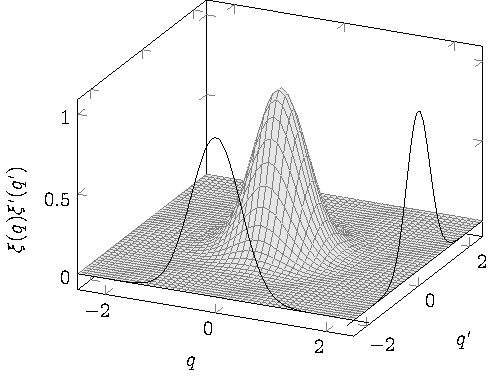
\includegraphics{diagrams/jpddemonstration}
    \caption{Example of the joint probability amplitude of a Gaussian wave packet.}
    \label{fig:jpddemonstration}
\end{figure}

\subsection{Interacting systems}

Let there be a state ket $\ket{\eta}$ which describes the quantum state of two particles. When the two particles are interacting, the time-evolution operator cannot be factored into tensor products of two operators. Therefore, there can only be one combined time-evolution operator for both of the systems:
\begin{equation}
    \hat{U}(t_F, t_0) = \exp[-\im\Dd{t}\left(\frac{\hat{p}^2}{2m} + \frac{\hat{p}'^2}{2m'} + V(\hat{q}, \hat{q}', t)\right)]
\end{equation}
The consequence of the combined time-evolution operator is that, we cannot calculate the joint probability distribution between different time of the subsystem. For simplicity’ sake, let the index $j = i + 1$, where $t_j = t_i + \Dd{t}$ in which $\Dd{t} \appr 0$.
\begin{align}
    &\braket{q_j, q_j'}{\eta(t_j)} \\
    &= \mel{q_j, q_j'}{\hat{U}(t_j, t_i)}{\eta(t_i)}. \\
    &= \iint \dd{q_i}\dd{q_i'} \mel{q_j, q_j'}{\hat{U}(t_j, t_i)}{q_i, q_i'}\braket{q_i, q_i'}{\eta(t_i)}.
\end{align}

As seen, the form of transition element is
\begin{equation}
    \mel{q_j, q_j'}{\exp[-\im\Dd{t}\left(\frac{\hat{p}^2}{2m} + \frac{\hat{p}'^2}{2m'} + V(\hat{q}, \hat{q}', t)\right)]}{q_i, q_i'}.
\end{equation}
The terms in the exponents can be separated due to the vanishing commutator when $\Dd{t} \appr 0$. By separating the terms in the exponents and inserting two complete sets of momentum basis, the equation above turns into
\begin{align}
    & \frac{1}{(2\cpi)^2} \iint\dd{p}\dd{p'} \mel*{q_j, q_j'}{\exp[-\im\Dd{t}\frac{\hat{p}^2}{2m}]}{p, p'}\mel{p, p'}{\exp[-\im\Dd{t}\frac{\hat{p}'^2}{2m'}]\exp[-\im\Dd{t}V(\hat{q}, \hat{q}', t)]}{q_i, q_i'} \nonumber\\
    &= \frac{1}{(2\cpi)^2} \iint\dd{p}\dd{p'} \exp[-iu\Dd{t}\left(\frac{p^2}{2m} + \frac{p'^2}{2m'} + V(q_i, q_i, \Dd{t})\right)]\braket{q_j}{p}\braket{q_j'}{p'}\braket{q_i}{p}\conj\braket{q_j'}{p'}\conj \nonumber\\
    &= \frac{1}{(2\cpi)^4} \e^{-\im\Dd{t}V(q_i, q_i', t)} \int\dd{p}\exp[-\im\Dd{t}\frac{p^2}{2m} + \im p(q_j - q_i)]\int\dd{p'}\exp[-\im\Dd{t}\frac{p'^2}{2m'} + \im p'(q_j' - q_i')^2] \nonumber\\
    &= \frac{(mm')^{\frac{1}{2}}}{8\cpi^3\im\Dd{t}}\exp[-\im\Dd{t}V(q_i, q_i', t) + \frac{\im m'}{2\Dd{t}}(q_j' - q_i')^2 + \frac{\im m}{2\Dd{t}}(q_j - q_i)^2].
\end{align}
To find the propagator for an interacting system, we need to perform successive integrals on $q$ and $q'$, i.e.,
\begin{equation}
    K_{\eta} = \idotsint \dd{q_N}\dd{q_N'}\dots\dd{q_1}\dd{q_1'}\mel{q_F, q_F'}{\hat{U}(t_F, t_N)}{q_N, q_N'}\dots\mel{q_1, q_1'}{\hat{U}(t_1, t_0)}{q_0, q_0'}
\end{equation}

Notice that when there is no interaction between the two systems ($V = 0$), the integrals become separable and reduces down to the form of the non-interacting system's propagator but off by a normalization factor.

There are two common forms of interaction, which is the spring interaction and the coulomb interaction. Both of which includes the term $(q_i - q_i')^2$ in $V(q, q')$, which causes major problems in integration. When expanded, there is a $q_iq_i'$ term that makes the integral inseparable which causes the integral pattern to not repeat; therefore, we resort to perturbation.

\subsection{Form of the two particle perturbation series}

The perturbation series for one particle are already given by Feynman in his path integrals textbook:
\begin{equation}
    K_n(F, 0) = \left(-\im\right)^n\idotsint K_0(F, n)\prod_{i = 1}^n V(i)K_0(i, i - 1)\dd{\tau_i}
\end{equation}
where $K_n$ is the $n$'th order perturbation, $K(j, k) = K(q_j, t_j; q_k, t_k)$, $K = \ssum_nK_n$ and $\dd{\tau_i} = \dd{q_i}\dd{q_i}\dd{t_i}$. To apply it with two particles, we extend it:
\begin{equation}
    K_n(F, 0; F', 0') = \left(-\im\right)^n\idotsint K_0(F, n)K_0(F', n')\left[\prod_{i = 1}^nV(i)K_0(i, i - 1)K_0(i', i' - 1)\dd{q_i}\dd{q_i'}\dd{t_i}\right]. \label{eq:generaltwoparticleperturbation}
\end{equation}
We can also expand the joint probability distribution in the form of the perturbation series.
\begin{align}
    \eta(q_F, q_F'; t_F) &= \int K(q_F, q_F'; q_0, q_0'; t_F - t_0)\eta(q_0, q_0'; t_0)\dd{q_0}\dd{q_0'} \\
    &= \int \sum_n K_n(q_F, q_F'; q_0, q_0'; t_F - t_0)\eta(q_0, q_0'; t_0) \dd{q_0}\dd{q_0'} \\
    &= \sum_n \int K_n(q_F, q_F'; q_0, q_0'; t_F - t_0)\eta(q_0, q_0'; t_0) \dd{q_0}\dd{q_0'}
\end{align}

\section{Initial states of choice}
\label{sec:initial_states_of_choice}

From now on, I shall use the letter $\xi$ to refer to a state of a single particle, and the letter $\eta$ to refer to the combined state of two particles.

We are interested in the time evolution of a Gaussian wave packet due to its mathematical simplicity. The normalized state of a Gaussian wave packet is given by
\begin{equation}
    \sqrt[4]{\frac{1}{2\cpi\sigma}}\exp[\im p q - \frac{(q - s)^2}{4\sigma^2}]. \label{eq:unentangled_state}
\end{equation}
For two separable particles, its joint probability is
\begin{align}
    \braket{q, q'}{\eta(t_0)} &= \sqrt[4]{\frac{1}{2\cpi\sigma^2}}\sqrt[4]{\frac{1}{2\cpi\sigma'^2}}\exp[\im pq - \frac{(q - s)^2}{4\sigma^2}]\exp[\im p'q' - \frac{(q' - s')^2}{4\sigma'^2}] \\
    &= \sqrt{\frac{1}{2\cpi\sigma\sigma'}}\exp[\im pq - \frac{(q - s)^2}{4\sigma^2}]\exp[\im p'q' - \frac{(q' - s')^2}{4\sigma'^2}]
\end{align}

As we'll see, the higher order perturbation terms (at least of the spring system) are expressed as the integral of the product between the wave function and some polynomials, which we'll find later.
\begin{align}
    &\braket{q}{\xi(t)} \\ &= \int K_0(q_F, q_0;t_F)\braket{q_0}{\xi(t)}\dd{q_0} \\
    &= \sqrt{\frac{m}{2\cpi\im t_F}}\int\exp[\frac{\im m}{2t_F}(q_F - q_0)^2] \left(\sqrt[4]{\frac{1}{2\cpi\sigma}}\exp[\im p q_0 - \frac{(q_0 - s)^2}{4\sigma^2}]\right)\dd{q_0} \\
    &= \sqrt[4]{-\frac{m^2}{8\cpi^3t_F^2\sigma^2}}\int\exp[\frac{\im m}{2t_F}(q_F - q_0)^2 + \im p q_0 - \frac{(q_0 - s)^2}{4\sigma^2}]\dd{q_0} \\
    &= \sqrt[4]{-\frac{m^2}{8\cpi^3t_F^2\sigma^2}}\int\exp[\left(\frac{\im m q_F^2}{2t_F} - \frac{s^2}{4\sigma^2}\right) + q\left(-\frac{\im m q_F}{t_F} + \im p + \frac{s}{2\sigma^2}\right) + q^2\left(\frac{\im m}{2t_F} - \frac{1}{4\sigma^2}\right)]\dd{q_0} \\
    &= \sqrt[4]{-\frac{m^2}{8\cpi^3t_F^2\sigma^2}} \cdot 2\sigma\sqrt{\frac{\cpi t_F}{-2\im m\sigma^2 + t_F}}\exp[\frac{4 \im m p q_{F} σ^{2} - m q_{F}^{2} + 2 m q_{F} s - m s^{2} - 2 \im p^{2} t_{F} σ^{2} - 2 p s t_{F}}{4 m σ^{2} + 2 \im t_{F}}]  \nonumber\\
    &= \sqrt[4]{\frac{2m^2\sigma^2}{\cpi(2m\sigma^2 + \im t_F)^2}}\exp[\frac{4 \im m p q_{F} σ^{2} - m q_{F}^{2} + 2 m q_{F} s - m s^{2} - 2 \im p^{2} t_{F} σ^{2} - 2 p s t_{F}}{4 m σ^{2} + 2 \im t_{F}}].
\end{align}
To plot its probability amplitude, we have to take its modulus squared, which equals to
\begin{equation}
    \frac{m σ}{\sqrt{4 m^{2} σ^{4} + t_{F}^{2}}}\exp[\frac{- 2 m^{2} q_{F}^{2} σ^{2} + 4 m^{2} q_{F} s σ^{2} - 2 m^{2} s^{2} σ^{2} + 4 m p q_{F} t_{F} σ^{2} - 4 m p s t_{F} σ^{2} - 2 p^{2} t_{F}^{2} σ^{2}}{4 m^{2} σ^{4} + t_{F}^{2}}]
\end{equation}

\section{The spring system}

The spring potential is given by $V(q, q') = \frac{k}{2}(q - q')^2$. I shall let $\alpha = \frac{k}{2}$ to simplify the notation a bit.

\subsection{First order perturbation term}
\label{sec:spring_1storder}

From \cref{eq:generaltwoparticleperturbation}, set $t_1 = t, t_0 = 0$
\begin{align}
    &K_1(F, 0; F', 0) \nonumber \\
    &= \left(-\im\right)^1\iiint K_0(F, 1)K_0(F', 1')K_0(1, 0)K_0(1, 0')\alpha(q_1 - q_1')^2\dd{q_1}\dd{q_1'}\dd{t}. \\
    &= -\im\alpha\int_0^{t_F}\left[\iint K_0(q_F, q_1; t_F - t)K_0(q_F', q_1'; t_F - t)K_0(q_1, q_0; t)K_0(q_1', q_0'; t)(q_1 - q_1')^2\dd{q_1}\dd{q_1'}\right]\dd{t}. \nonumber
\end{align}
We then let the terms in the square bracket,
\begin{equation}
    \iint K_0(q_F, q_1; t_F - t)K_0(q_F', q_1'; t_F - t)K_0(q_1, q_0; t)K_0(q_1', q_0'; t)(q_1 - q_1')^2\dd{q_1}\dd{q_1'}
\end{equation}
equals $I$; therefore, $K_1 = -\im\alpha\int_0^{t_F} I\dd{t}$.

We then separate $I$ into three integrals:
\begin{gather}
    I_{P1} = \int q_1^2K_0(q_F, q_1; t_F - t)K_0(q_1, q_0; t)\dd{q_1} \int K_0(q_F', q_1'; t_F - t)K_0(q_1', q_0'; t)\dd{q_1'}, \label{eq:spring_IP1}\\
    I_{P2} = \int K_0(q_F, q_1; t_F - t)K_0(q_1, q_0; t)\dd{q_1} \int q_1'^2K_0(q_F', q_1'; t_F - t)K_0(q_1', q_0'; t)\dd{q_1'}, \label{eq:spring_IP2}\\
    I_{P3} = \int q_1K_0(q_F, q_1; t_F - t)K_0(q_1, q_0; t)\dd{q_1} \int q_1'K_0(q_F', q_1'; t_F - t)K_0(q_1', q_0'; t) \dd{q_1'} \label{eq:spring_IP3},
\end{gather}
where $I = I_{P1} + I_{P2} + 2I_{P3}$. The integrals without the factor $q_1$ and $q_1^2$ can be reduced into the kernel for the free particle:
\begin{gather}
    I_{P1} = K_0(q_F', q_0'; t_F)\int q_1^2K_0(q_F, q_1; t_F - t)K_0(q_1, q_0; t)\dd{q_1} \\
    I_{P2} = K_0(q_F, q_0; t_F)\int q_1'^2 K_0(q_F', q_1'; t_F - t)K_0(q_1', q_0'; t)\dd{q_1'}
\end{gather}
Since $I_{P2}$ can be obtained by switching all the primed variables with the corresponding unprimed in $I_{P1}$, we're left with two family of integrals:
\begin{equation}
    \int q_1K_0(q_F, q_1; t_F - t)K_0(q_1, q_0; t)\dd{q_1} \mathand \int q_1^2K_0(q_F, q_1; t_F - t)K_0(q_1, q_0; t)\dd{q_1}. \label{eq:spring_family_of_integrals}
\end{equation}
To evaluate these, we first simplify the product of kernel under the assumption that $t_F > t$.
\begin{align}
    &K_0(q_F, q_1; t_F - t)K_0(q_1, q_0; t) \nonumber\\
    &= \sqrt{\frac{m}{2\cpi\im(t_F - t)}}\sqrt{\frac{m}{2\cpi\im t}}\exp[\frac{\im m}{2(t_F - t)}(q_F - q_1)^2 + \frac{\im m}{2t}(q_1 - q_0)^2] \\
    &= \frac{m}{2\cpi}\sqrt{-\frac{1}{t(t_F - t)}} \exp[q_1^2\left(\frac{\im m}{2t} + \frac{\im m}{2(t_F - t)}\right) - q_1\left(\frac{\im m q_0}{t} + \frac{\im m q_F}{t_F - t}\right) + \left(\frac{\im m q_0^2}{2t} + \frac{\im m q_F^2}{2(t_F - t)}\right)] \nonumber \\
    &= \frac{m}{2\cpi}\sqrt{-\frac{1}{t(t_F - t)}} \exp[-q_1^2\left(\frac{m t_F}{2\im t(t_F - t)}\right) - q_1(\im m)\left(\frac{q_0}{t} + \frac{q_F}{t_F - t}\right) - \left(\frac{m}{2\im}\right)\left(\frac{q_0^2}{t} + \frac{q_F^2}{t_F - t}\right)] \nonumber
\end{align}
The normalization factor are pulled out. Both integrals in \cref{eq:spring_family_of_integrals} can be evaluated with
\begin{equation}
    a = \frac{m t_F}{2\im t(t_F - t)}, \quad b = \im m\left(\frac{q_0}{t} + \frac{q_F}{t_F - t}\right) \mathand c = \left(\frac{m}{2\im}\right)\left(\frac{q_0^2}{t} + \frac{q_F^2}{t_F - t}\right)
\end{equation}
in which,
\begin{equation}
    \exp[\frac{b^2}{4a} - c] = \exp[\frac{\im m}{2t_F}(q_F - q_0)^2] = \sqrt{\frac{2\cpi\im t_F}{m}}K_0(q_F, q_0; t_F).
\end{equation}
To summarize,
\begin{align}
    \int q_1K_0(q_F, q_1; t_F - t)K_0(q_1, q_0; t)\dd{q_1} &= -\frac{b}{2}\sqrt{\frac{\cpi}{a^3}}\times\frac{m}{2\cpi}\sqrt{-\frac{1}{t(t_F - t)}}\times\sqrt{\frac{2\cpi\im t_F}{m}}K_0(q_F, q_0; t_F) \nonumber\\
    &= -\frac{b}{2}\sqrt{\frac{\cpi}{a^3}} \times \sqrt{\frac{mt_F}{2\cpi\im t(t_F - t)}}K_0(q_F, q_0; t_F), \label{eq:spring_deg1gaussian_form}
\end{align}
and
\begin{equation}
    \int q_1^2K_0(q_F, q_1; t_F - t)K_0(q_1, q_0; t)\dd{q_1} = \frac{1}{4}\sqrt{\frac{\cpi}{a^5}}(2a + b^2) \times \sqrt{\frac{mt_F}{2\cpi\im t(t_F - t)}}K_0(q_F, q_0; t_F). \label{eq:spring_deg2gaussian_form}
\end{equation}

On the Gaussian integral with degree one,
\begin{equation}
    -\frac{b}{2}\sqrt{\frac{\cpi}{a^3}} = \sqrt{\frac{2\cpi t}{mt_F^3}}\frac{\sqrt{-\im(t_F - t)^3}}{\im(t_F - t)} \times \left[q_0(t_F - t) + q_Ft\right];
\end{equation}
thus from \cref{eq:spring_deg1gaussian_form},
\begin{align}
    \int q_1K_0(q_F, q_1; t_F - t)K_0(q_1, q_0; t) &= \begin{multlined}[t]
        \sqrt{\frac{2\cpi t}{mt_F^3}}\frac{\sqrt{-\im(t_F - t)^3}}{\im(t_F - t)} \times \left[q_0(t_F - t) + q_Ft\right] \\
        \times \sqrt{\frac{mt_F}{2\cpi\im t(t_F - t)}}K_0(q_F, q_0; t_F)
    \end{multlined} \\
    &= -\frac{1}{t_F}\left[q_0(t_F - t) + q_Ft\right]K_0(q_F, q_0; t_F).
\end{align}
On the Gaussian integral with degree two,
\begin{equation}
    \frac{1}{4}\sqrt{\frac{\cpi}{a^5}}(2a + b^2) = -\sqrt{\frac{2\cpi t}{m^3t_F^5}}\frac{\sqrt{\im(t_F - t)^5}}{(t_F - t)^2}\left[m\left(q_0(t_F - t) + q_Ft\right)^2 + \im tt_F(t_F - t)\right];
\end{equation}
and thus,
\begin{align}
    &\int q_1^2K_0(q_F, q_1; t_F - t)K_0(q_1, q_0; t)\dd{q_1} \\
    &= \sqrt{\frac{mt_F}{2\cpi\im t(t_F - t)}}K_0(q_F, q_0; t_F)  \times -\sqrt{\frac{2\cpi t}{m^3t_F^5}}\frac{\sqrt{\im(t_F - t)^5}}{(t_F - t)^2}\left[m\left(q_0(t_F - t) + q_Ft\right)^2 + \im tt_F(t_F - t)\right] \nonumber\\
    &= -\frac{1}{mt_F^2}\left[m\left(q_0(t_F - t) + q_Ft\right)^2 + \im tt_F(t_F - t)\right]K_0(q_F, q_0; t_F).
\end{align}

We're now in the place to finally construct the first order propagator term for the spring system. Recall that
\begin{equation}
    K_1 = -\im\alpha\int_0^{t_F} I\dd{t} = -\im\alpha\left[\int_0^{t_F}I_{P1}\dd{t} + \int_0^{t_F}I_{P2}\dd{t} + 2\int_0^{t_F}I_{P3}\dd{t}\right]
\end{equation}
From earlier,
\begin{gather}
    \begin{aligned}
        I_{P1} &= K_0(q_F', q_0'; t_F)\int q_1^2K_0(q_F, q_1; t_F - t)K_0(q_1, q_0; t)\dd{q_1} \\
        &= -\frac{1}{mt_F^2}\left[m\left(q_0(t_F - t) + q_Ft\right)^2 + \im tt_F(t_F - t)\right]K_0(q_F, q_0; t_F)K_0(q_F', q_0'; t_F),
    \end{aligned}
    \\
    \begin{aligned}
        I_{P2} &= K_0(q_F, q_0; t_F)\int q_1'^2 K_0(q_F', q_1'; t_F - t)K_0(q_1', q_0'; t)\dd{q_1'} \\
        &= -\frac{1}{mt_F^2}\left[m\left(q_0'(t_F - t) + q_F't\right)^2 + \im tt_F(t_F - t)\right]K_0(q_F, q_0; t_F)K_0(q_F', q_0'; t_F),
    \end{aligned}
    \\
    \begin{aligned}
        I_{P3} &= -\frac{1}{t_F}\left[q_0(t_F - t) + q_Ft\right]K_0(q_F, q_0; t_F) \times -\frac{1}{t_F}\left[q_0'(t_F - t) + q_F't\right]K_0(q_F', q_0'; t_F) \\
        &= \frac{1}{t_F^2}\left[q_0(t_F - t) + q_Ft\right]\left[q_0'(t_F - t) + q_F't\right]K_0(q_F, q_0; t_F)K_0(q_F', q_0'; t_F).
    \end{aligned}
\end{gather}
Thus,
\begin{multline}
    K_1 = -\im\alpha K_0(q_F, q_0; t_F)K_0(q_F', q_0'; t_F) \frac{1}{t_F^2} \left[-\frac{1}{m}\int_0^{t_F}m\left(q_0(t_F - t) + q_Ft\right)^2 + \im tt_F(t_F - t)\dd{t} \right. \\
    -\frac{1}{m}\int_0^{t_F}m\left(q_0'(t_F - t) + q_F't\right)^2 + \im tt_F(t_F - t)\dd{t} \\
    \left. + \int_0^{t_F}\left[q_0(t_F - t) + q_Ft\right]\left[q_0'(t_F - t) + q_F't\right]\dd{t}\right]
\end{multline}
The integrals are then taken out to be evaluated term by term. Since the integrand of these integrals are all polynomials, we can just plug it into \texttt{SymPy.jl}:
\begin{gather}
    \int_0^{t_F}m\left(q_0(t_F - t) + q_Ft\right)^2 = \frac{t_F^3}{6}\left(2m(q_0 + q_F)^2 + \im t_F\right) \\
    \int_0^{t_F}m\left(q_0'(t_F - t) + q_F't\right)^2 = \frac{t_F^3}{6}\left(2m(q_0' + q_F')^2 + \im t_F\right) \\
    \int_0^{t_F}\left[q_0(t_F - t) + q_Ft\right]\left[q_0'(t_F - t) + q_F't\right]\dd{t} = \frac{t_F^3}{6}\left(2q_0q_0' + q_0q_F' + q_0'q_F + 2q_Fq_F'\right)
\end{gather}
Therefore, the first order perturbation term of the spring system takes the form
\begin{multline}
    K_1(q_F, q_0; q_F', q_0'; t_F) = -\im\frac{\alpha t_F}{6}K_0(q_F, q_0; t_F)K_0(q_F', q_0'; t_F) \\
    \times\left[-2\left(m(q_0 + q_F)^2 + m(q_0' + q_F')^2 + \im t_F\right) + 2q_0q_0' + q_0q_F' + q_0'q_F + 2q_Fq_F'\right]. \label{eq:spring_first_order_perturbation}
\end{multline}

\paragraph{Interpretation of the propagator} As of now, my knowledge of the propagator is pretty limited.

\subsection{Joint probability contribution from the first order perturbation term}

Let us first analyze the time evolution of a separable wave packet with the initial state
\begin{equation}
    \eta(q_0, q_0; t_0) \equiv \frac{1}{2\cpi\sqrt{\sigma\sigma'}}\exp[\im pq_0 + \im p'q_0' - \frac{(q_0 - s)^2}{4\sigma^2} - \frac{(q_0' - s')^2}{4\sigma'^2}].
\end{equation}
For simplicity's sake, let
\begin{gather*}
    \xi \equiv \exp[\im pq_0 - \frac{(q_0 - s)^2}{4\sigma^2}], \quad \xi' \equiv \exp[\im p'q_0' - \frac{(q_0' - s')^2}{4\sigma'^2}], \\
    K \equiv \sqrt{\frac{m}{2\cpi\im t_F}}\exp[\frac{\im}{2t_F}(q_F - q_0)^2], \quad K' \equiv \sqrt{\frac{m}{2\cpi\im t_F}}\exp[\frac{\im}{2t_F}(q_F' - q_0')^2].
\end{gather*}
Let us also set $t_0$ to be $0$. Using the first order perturbation term from \cref{eq:spring_first_order_perturbation}, the state at any following time $t_F$ is then
\begin{align}
    \eta(q_F, q_F'; t_F) &= \iint\left(K_0(q_F, q_0; q_F', q_0'; t_F - t_0) + K_1(q_F, q_0; q_F', q_0'; t_F - t_0)\right)\eta(q_0, q_0'; t_0)\dd{q}\dd{q_0'} \\
    &= \begin{multlined}[t]
        \frac{1}{2\cpi\sqrt{\sigma\sigma'}}\iint K_0(q_F, q_0; q_F', q_0'; t_F - t_0)\left\{1 - \im\frac{\alpha t_F}{6}\left[-2\left(m(q_0 + q_F)^2 \right.\right.\right.\\
        \left.\left.\left. + m(q_0' + q_F')^2 + \im t_F\right) + 2q_0q_0' + q_0q_F' + q_0'q_F + 2q_Fq_F'\right]\vphantom{\frac{\alpha t_F}{6}}\right\}
        \\ \exp[\im pq_0 + \im p'q_0' - \frac{(q_0 - s)^2}{4\sigma^2} - \frac{(q_0' - s')^2}{4\sigma'^2}]\dd{q_0}\dd{q_0'}
    \end{multlined} \\
    &= \begin{multlined}[t]
        \frac{1}{2\cpi\sqrt{\sigma\sigma'}}\iint KK'\xi\xi'\left\{1 - \im\frac{\alpha t_F}{6}\left[-2\left(m(q_0 + q_F)^2 \right.\right.\right.\\
        \left.\left.\left. + m(q_0' + q_F')^2 + \im t_F\right) + 2q_0q_0' + q_0q_F' + q_0'q_F + 2q_Fq_F'\right]\vphantom{\frac{\alpha t_F}{6}}\right\} \dd{q_0}\dd{q_0'}
    \end{multlined}
\end{align}
Note that this method of separation will work for all separable $\eta(t_0)$. Therefore, $\eta(t_0)$ doesn't have to be Gaussian: we just select it to be. The integral above can then be further expanded and broken down into smaller integrals:
\begin{align}
    \eta(q_F, q_F'; t_F) &= \begin{multlined}[t]
        \frac{1}{2\cpi\sqrt{\sigma\sigma'}}\left[\iint KK'\xi\xi'\dd{q_0}\dd{q_0'} \right.\\ \left.
        - \im\frac{\alpha t_F}{6}\iint KK'\xi\xi'\Big\{-2m(q_0^2 + 2q_0q_F + q_F^2 + q_0'^2 + 2q_0'q_F' + q_F'^2) \right.\\ \left.
        + 2q_0q_0' + 2q_Fq_F' + q_0q_F' + q_0'q_F + \im t_F\Big\}\dd{q_0}\dd{q_0'}  \vphantom{\iint}\right]
    \end{multlined} \\
\end{align}
I shall let $I$ equals the term in the big square bracket:
\begin{equation}
    I \equiv \begin{multlined}[t]
        \iint KK'\xi\xi'\dd{q_0}\dd{q_0'}
        - \im\frac{\alpha t_F}{6}\iint KK'\xi\xi'\Big\{-2m(q_0^2 + 2q_0q_F + q_F^2 + q_0'^2 + 2q_0'q_F' + q_F'^2) \\
        + 2q_0q_0' + 2q_Fq_F' + q_0q_F' + q_0'q_F + \im t_F\Big\}\dd{q_0}\dd{q_0'}
    \end{multlined}
\end{equation}
and thus,
\begin{equation}
    \eta(q_F, q_F'; t_F) \equiv \frac{1}{2\cpi\sqrt{\sigma\sigma'}}I 
\end{equation}
We then pull the terms that doesn't include $q_0$ or $q_0'$ out:
\begin{align}
    I &= \begin{multlined}[t]
        \left[\iint KK'\xi\xi'\dd{q_0}\dd{q_0}\right]
        + \left[\iint KK'\xi\xi'\dd{q_0}\dd{q_0}\right]\left(-\im\frac{\alpha t_F}{6}\right)\left(-2m(q_F^2 + q_F'^2) + 2q_Fq_F' + \im t_F\right) \\
        - \left(\frac{\im\alpha t_F}{6}\right)\iint KK'\xi\xi'\left\{-2m(q_0^2 + q_0'^2 + 2q_0q_F + 2q_0'q_F') + 2q_0q_0' + q_0q_F' + q_0'q_F\right\}\dd{q_0}\dd{q_0}
    \end{multlined} \nonumber \\
    &= \begin{multlined}[t]
        \left[\iint KK'\xi\xi'\dd{q_0}\dd{q_0}\right]\left[1 + \left(\frac{\im\alpha t_F}{6}\right)\left(2m(q_F^2 + q_F'^2) - 2q_Fq_F' - \im t_F\right)\right] \\
        - \left(\frac{\im\alpha t_F}{6}\right)\left[\iint KK'\xi\xi'\left\{-2m(q_0^2 + q_0'^2 + 2q_0q_F + 2q_0'q_F') + 2q_0q_0' + q_0q_F' + q_0'q_F\right\}\dd{q_0}\dd{q_0}\right]
    \end{multlined} \nonumber\\
    &= \begin{multlined}[t]
        \left[\int K\xi\dd{q_0}\int K'\xi'\dd{q_0'}\right]\left[1 + \left(\frac{\im\alpha t_F}{6}\right)\left(2m(q_F^2 + q_F'^2) - 2q_Fq_F' - \im t_F\right)\right] \\
        - \left(\frac{\im\alpha t_F}{6}\right) \left\{-2m\left[\int q_0^2K\xi\dd{q_0}\int K\xi'\dd{q_0'} + \int K\xi\dd{q_0}\int q_0'^2K'\xi'\dd{q_0'}\right] \right. \\
        -4mq_F\left[\int q_0K\xi\dd{q_0}\int K\xi'\dd{q_0'} + \int K\xi\dd{q_0}\int q_0'K'\xi'\dd{q_0'}\right] \\
        + q_F\left[\int K\xi\dd{q_0}\int q_0'K'\xi'\dd{q_0'}\right] + q_F'\left[\int q_0K\xi\dd{q_0}\int K\xi'\dd{q_0'}\right] \\ \left.
        + 2\left[\int q_0K\xi\dd{q_0}\int q_0'K\xi'\dd{q_0'}\right] \right\}
    \end{multlined}
\end{align}
For the purpose of legibility, let
\begin{multline}
    I_0 = \int K\xi\dd{q_0}, \quad I_1 = \int q_0K\xi\dd{q_0}, \quad I_2 = \int q_0^2K\xi\dd{q_0}, \\
    I_0' = \int K'\xi'\dd{q_0'}, \quad I_1' = \int q_0'K'\xi'\dd{q_0'} \mathand I_2' = \int q_0'^2K'\xi'\dd{q_0'}. \label{eq:integral_components_spring_jpd}
\end{multline}
Thus, $I$; and hence $\eta$, becomes
\begin{equation}
    \eta(q_F, q_F'; t_F) = \begin{multlined}[t]
        \frac{1}{2\cpi\sqrt{\sigma\sigma'}}\left\{I_0I_0'\left[1 + \left(\frac{\im\alpha t_F}{6}\right)\left(2m(q_F^2 + q_F'^2) - 2q_Fq_F' - \im t_F\right)\right] \right. \\ \left.
        - \left(\frac{\im\alpha t_F}{6}\right) \left[-2m\left(I_2I_0' + I_0I_2'\right) - 4mq_F\left(I_1I_0' + I_0I_1'\right) + q_FI_0I_1' + q_F'I_1I_0' + 2I_1I_1' \right] \right\}
    \end{multlined}
\end{equation}
As said earlier, this equation is general for the spring propagator with separable initial state. When $\alpha = 0$, this joint probability distribution reduces down to the joint probability distribution for the free particle.

The integrals listed in \cref{eq:integral_components_spring_jpd} are then evaluated:
\begin{gather}
    I_0 = \int K\xi\dd{q_0} = \sqrt{\frac{m}{2\cpi\im t_F}}\sqrt[4]{\frac{1}{2\cpi\sigma}} \int \exp[\im pq_0 - \frac{(q_0 - s)^2}{4\sigma^2} + \frac{\im m}{2t_F}(q_F - q_0)^2]\dd{q_0} \\
    I_1 = \int q_0K\xi\dd{q_0} = \sqrt{\frac{m}{2\cpi\im t_F}}\sqrt[4]{\frac{1}{2\cpi\sigma}} \int q_0\exp[\im pq_0 - \frac{(q_0 - s)^2}{4\sigma^2} + \frac{\im m}{2t_F}(q_F - q_0)^2]\dd{q_0} \\
    I_2 = \int q_0^2K\xi\dd{q_0} = \sqrt{\frac{m}{2\cpi\im t_F}}\sqrt[4]{\frac{1}{2\cpi\sigma}} \int q_0^2\exp[\im pq_0 - \frac{(q_0 - s)^2}{4\sigma^2} + \frac{\im m}{2t_F}(q_F - q_0)^2]\dd{q_0}
\end{gather}
All of these integrals are Gaussian integrals with the exponential argument
\begin{align}
    &\im pq_0 - \frac{(q_0 - s)^2}{4\sigma^2} + \frac{\im m}{2t_F}(q_F - q_0)^2 \\
    &= -\left(\frac{1}{4\sigma^2} - \frac{\im m}{2t_F}\right)q_0^2 - \left(\frac{\im m q_F}{t_F} - \im p - \frac{s}{2\sigma^2}\right)q_0 - \left(\frac{s^2}{4\sigma^2} - \frac{\im m q_F^2}{2t_F}\right),
\end{align}
with
\begin{equation}
    a = \frac{1}{4\sigma^2} - \frac{\im m}{2t_F}, \quad b = \frac{\im m q_F}{t_F} - \im p - \frac{s}{2\sigma^2} \mathand \frac{s^2}{4\sigma^2} - \frac{\im m q_F^2}{2t_F}.
\end{equation}
From \cref{sec:initial_states_of_choice},
\begin{equation}
    \exp[\frac{b^2}{4a} - c] = \exp[\frac{4 \im m p q_{F} σ^{2} - m q_{F}^{2} + 2 m q_{F} s - m s^{2} - 2 \im p^{2} t_{F} σ^{2} - 2 p s t_{F}}{4 m σ^{2} + 2 \im t_{F}}].
\end{equation}
I shall let
\begin{gather}
    \Xi \equiv \sqrt{\frac{m}{2\cpi\im t_F}}\sqrt[4]{\frac{1}{2\cpi\sigma}}\exp[\frac{4 \im m p q_{F} σ^{2} - m q_{F}^{2} + 2 m q_{F} s - m s^{2} - 2 \im p^{2} t_{F} σ^{2} - 2 p s t_{F}}{4 m σ^{2} + 2 \im t_{F}}], \\
    \Xi' \equiv \sqrt{\frac{m}{2\cpi\im t_F}}\sqrt[4]{\frac{1}{2\cpi\sigma'}}\exp[\frac{4 \im m p' q_F' σ'^2 - m q_F'^2 + 2 m q_{F}'s' - ms'^{2} - 2 \im p'^2t_Fσ'^{2} - 2p's't_F}{4m'σ'^2 + 2\im t_{F}}]
\end{gather}
which represents the unperturbed state of a particle. And,
\begin{gather}
    \sqrt{\frac{\cpi}{a}} = 2\sigma\sqrt{\frac{\cpi t_F}{t_F - 2\im m\sigma^2}} \equiv G_0, \\
    -\frac{b}{2}\sqrt{\frac{\cpi}{a^3}} = 2\sigma\sqrt{\frac{\cpi t_F}{(t_F - 2\im m\sigma^2)^3}}\left(-2\im q_F + 2\im p t_F\sigma^2 + st_F\right) \equiv G_1, \\
    \frac{1}{4}\sqrt{\frac{\cpi}{a^5}} = 2\sigma\sqrt{\frac{\cpi t_F}{(t_F - 2\im m\sigma^2)^5}}\left(- 4 \im m t_{F} σ^{4} + 2 t_{F}^{2} σ^{2} + \left(- 2 \im m q_{F} σ^{2} + 2 \im p t_{F} σ^{2} + s t_{F}\right)^{2}\right) \equiv G_2.
\end{gather}
Therefore, with the change of primed and unprimed variables,
\begin{equation}
    I_0 = G_0\Xi, \quad I_1 = G_1\Xi, \quad I_2 = G_2\Xi, \quad
    I_0' = G_0'\Xi', \quad I_1' = G_1'\Xi', \mathand I_2' = G_2'\Xi'
\end{equation}
$\eta$ then becomes
\begin{align}
    \eta &= \begin{multlined}[t]
        \frac{1}{2\cpi\sqrt{\sigma\sigma'}}\left\{ G_0G_0'\Xi\Xi'\left[1 + \left(\frac{\im\alpha t_F}{6}\right)\left(2m(q_F^2 + q_F'^2) - 2q_Fq_F' - \im t_F\right)\right] \right.\\
        - \left(\frac{\im\alpha t_F}{6}\right) \left[-2m\left(G_2G_0'\Xi\Xi' + G_0G_2'\Xi\Xi'\right) - 4mq_F\left(G_1G_0'\Xi\Xi' + G_0G_1'\Xi\Xi'\right) \right. \\ \left.\left.
        + q_FG_0G_1'\Xi\Xi' + q_F'G_1G_0'\Xi\Xi' + 2G_1G_1'\Xi\Xi'\right] \vphantom{\frac{1}{2\cpi\sqrt{\sigma\sigma'}}}\right\}
    \end{multlined} \\
    &= \begin{multlined}[t]
        \frac{\Xi\Xi'}{2\cpi\sqrt{\sigma\sigma'}}\left\{ G_0G_0'\left[1 + \left(\frac{\im\alpha t_F}{6}\right)\left(2m(q_F^2 + q_F'^2) - 2q_Fq_F' - \im t_F\right)\right] \right.\\ \left.
        - \left(\frac{\im\alpha t_F}{6}\right) \left[-2m\left(G_2G_0' + G_0G_2'\right) - 4mq_F\left(G_1G_0' + G_0G_1'\right)
        + q_FG_0G_1' + q_F'G_1G_0' + 2G_1G_1'\right] \vphantom{\frac{1}{2\cpi\sqrt{\sigma\sigma'}}}\right\}
    \end{multlined} \nonumber\\
    &= \begin{multlined}[t]
        \frac{\Xi\Xi'}{2\cpi\sqrt{\sigma\sigma'}} \left\{ G_0G_0'\left[1 + \left(\frac{\im\alpha t_F}{6}\right) \left( 2m(q_F^2 + q_F'^2) - 2q_Fq_F' - \im t_F\right)\right] \right. \\ \left.
        - \left(\frac{\im\alpha t_F}{6}\right) \left[G_0(q_FG_1'(1 - 4m) - 2mG_2') + G_0'(q_FG_1(1 - 4m) - 2mG_2) + 2G_1G_1'\right] \right\}
    \end{multlined}
\end{align}

We then proceed to normalize the state $\eta$

\subsection{Entanglement entropy}

\subsection{Joint probability contribution from the first order perturbation term on an entangled state}

\subsection{Second order perturbation term}

The second order perturbation term, $K_2$ is
\begin{align}
    K_2 &= \idotsint K_0(F, 2)V(2)K_0(2, 1)V(1)K_0(1, 0)\dd{q_1}\dd{q_1'}\dd{t_1}\dd{q_2}\dd{q_2'}\dd{t_2} \\
    &= \begin{multlined}[t]
        \idotsint K_0(q_F, q_2; t_F - t_2)K_0(q_F', q_2'; t_F - t_2)K_0(q_2, q_1; t_2 - t_1)K_0(q_2, q_1; t_2 - t_1) \\ \times K_0(q_1, q_0; t_1 - t_0)K_0(q_1, q_0; t_1 - t_0)(q_2 - q_2')^2(q_1 - q_1')^2\dd{q_1}\dd{q_1'}\dd{t_1}\dd{q_2}\dd{q_2'}\dd{t_2}
    \end{multlined} \\
    &= \begin{multlined}[t]
        \int_{t_1}^{t_F}\int_{t_0}^{t_F}\left[\idotsint K_0(q_F, q_2; t_F - t_2)K_0(q_F', q_2'; t_F - t_2)K_0(q_2, q_1; t_2 - t_1)\right. \\ \times K_0(q_2, q_1; t_2 - t_1)K_0(q_1, q_0; t_1 - t_0)K_0(q_1, q_0; t_1 - t_0) \left(\vphantom{\left(q_{2}^{\prime}\right)^{2}} q_{1}^{2} q_{2}^{2} - 2 q_{1}^{2} q_{2} q_{2}^{\prime} \right.\\ + q_{1}^{2} \left(q_{2}^{\prime}\right)^{2} - 2 q_{1} q_{2}^{2} q_{1}^{\prime} + 4 q_{1} q_{2} q_{1}^{\prime} q_{2}^{\prime} - 2 q_{1} q_{1}^{\prime} \left(q_{2}^{\prime}\right)^{2} + q_{2}^{2} \left(q_{1}^{\prime}\right)^{2} \\ \left.\left. - 2 q_{2} \left(q_{1}^{\prime}\right)^{2} q_{2}^{\prime} + \left(q_{1}^{\prime}\right)^{2} \left(q_{2}^{\prime}\right)^{2} \right) \dd{q_1}\dd{q_1'}\dd{q_2}\dd{q_2'} \vphantom{\idotsint}\right]\dd{t_1}\dd{t_2}
    \end{multlined}
\end{align}
The integral once again can be broken into nine integrals that must be integrated w.r.t. time twice later on. All those nine integrals have a product of propagator as a multiplier. We shall evaluate those first, separating the primed and unprimed variables.
\begin{align}
    &\begin{multlined}[t]
        K_0(q_F, q_2; t_F - t_2)K_0(q_F', q_2'; t_F - t_2)K_0(q_2, q_1; t_2 - t_1)K_0(q_2, q_1; t_2 - t_1)K_0(q_1, q_0; t_1 - t_0) \\ \times K_0(q_1, q_0; t_1 - t_0)
    \end{multlined} \nonumber \\
    &= \begin{multlined}[t]
        \frac{\im m^3}{8\cpi^3(t_F - t_2)(t_2 - t_1)(t_1 - t_0)}\exp \left[\frac{\im m}{2(t_F - t_2)}\left((q_F - q_2)^2 + (q_F' - q_2')^2\right) \right. \\ \left. + \frac{\im m}{2(t_2 - t_1)}\left((q_2 - q_1)^2 + (q_2' - q_1')^2\right) + \frac{\im m}{2(t_1 - t_0)}\left((q_1 - q_0)^2 + (q_1' - q_0')^2\right)\right]
    \end{multlined}
\end{align}

% \section{The delta function collision problem}

% The potential for the delta function collision problem is
% \begin{equation}
%     V = V_0\ddel(q - q')
% \end{equation}
% where $V_0$ is the strength of the delta function, and is generally considered to be negative.

% \subsection{First order perturbation term}

% We evaluate the perturbation term similarly to how we did it in \cref{sec:spring_1storder}, starting with the form:
% \begin{align}
%     &K_1(F, 0; F', 0) \\
%     &= -\im\int_0^{t_F}\left[\iint K_0(q_F, q_1; t_F - t)K_0(q_F', q_1'; t_F - t)K_0(q_1, q_0; t)K_0(q_1', q_0'; t)V_0\ddel(q_1 - q_1')\dd{q_1}\dd{q_1'}\right]\dd{t}. \nonumber \\
%     &= -\im V_0\int_0^{t_F}\left[\iint K_0(q_F, q_1; t_F - t)K_0(q_F', q_1'; t_F - t)K_0(q_1, q_0; t)K_0(q_1', q_0'; t)\ddel(q_1 - q_1')\dd{q_1}\dd{q_1'}\right]\dd{t} \nonumber
% \end{align}
% Let $I_1$ represents the integral in the square bracket; thus, $K_1 = -\im V_0\int_{0}^{t_F}I_1\dd{t}$. Then,
% \begin{align}
%     I_1 &= \iint K_0(q_F, q_1; t_F - t)K_0(q_F', q_1'; t_F - t)K_0(q_1, q_0; t)K_0(q_1', q_0'; t)\ddel(q_1 - q_1')\dd{q_1}\dd{q_1'} \\
%     &= \int K_0(q_F, q_1'; t_F - t)K_0(q_F', q_1'; t_F - t)K_0(q_1', q_0; t)K_0(q_1', q_0'; t)\dd{q_1'} \\
%     &= 
% \end{align}

\section{Anharmonic oscillator}

An anharmonic oscillator's potential is in the form
\chapter{Path integrals for bipartite system in the momentum basis}
\label{sec:perturbation_series_momentum}

\section{Relations between the position and momentum propagator}
\include{chapters/thefourierbasis}
\chapter{Correlation function}
\chapter{Implementation of simulations}
\label{sec:implementation_of_simulation}

To represent the joint probability distribution of a two particle system, we need four axes. Two for the position of each Hilbert space that those particles belong in, one for the probability amplitude, and one for the time.
\begin{align}
    P(q_F, q_F'; t_F) &= |\braket{q_F, q_F'}{\eta(t_F)}|^2 \\
    &= \left|\iint K(q_F, q_F', t_F; q_0, q_0', t_0)\eta(q_0, q_0', t_0)\dd{q_0}\dd{q_0'}\right|^2 \\
    &= \left|\iint \left\{\sum_{i = 0}^{\infty}K_i(q_F, q_F', t_F; q_0, q_0', t_0)\right\}\eta(q_0, q_0', t_0)\dd{q_0}\dd{q_0'}\right|^2 \\
    \intertext{For this equation to work with a discrete simulation, we need to exchange the integral sign with the summation sign:}
    &= \left|\sum_{\vphantom{q_0'}q_0}\sum_{q_0'}\left\{\sum_{\vphantom{q_0'}i = 0}^{\infty}K_i(q_F, q_F', t_F; q_0, q_0', t_0)\right\}\eta(q_0, q_0', t_0)\right|
\end{align}
The sum of propagators can then be truncated to our liking. I've written the code in \texttt{Julia} to test for the free particle propagator, and it looks something like this:
\begin{minted}{julia}
using Plots; plotlyjs()
using LinearAlgebra
using SymPy
using BenchmarkTools

q, q0, q1, q2, qf = symbols("q q_0 q_1 q_2 q_F", real = true)
m, t, t0, t1, t2, tf = symbols("m t t_0 t_1 t_2 t_F", real = true, positive = true)
q0p, q1p, q2p, qfp = symbols("q^{\\prime}_0 q^{\\prime}_1 q^{\\prime}_2 q^{\\prime}_F", real = true)
a, b, c, d, e, f = symbols("a b c d e f")
s1, s2, p1, p2, σ1, σ2 = symbols("s_1 s_2 p_1 p_2 σ_1 σ_2")

freePropagator(finPos, startPos, finTime, startTime = 0, m = 1) = sqrt(m / (2 * pi * im * (finTime - startTime))) * exp(im * m / (2 * (finTime - startTime)) * (finPos - startPos)^2)  
freePropagatorC(qf, qfp, q0, q0p, tf, t0) = freePropagator(qf, q0, tf, t0) + freePropagator(qfp, q0p, tf, t0)

initStateFunction(q0, q0p, σ1, s1, p1, σ2, s2, p2) = (1//2 * pi * σ1)^(1//4) * exp(-(q0 - s1)^2 / (4 * σ1^2) + im * p1 * q0) * (1//2 * pi * σ2)^(1//4) * exp(-(q0p - s2)^2 / (4 * σ2^2) + im * p2 * q0p)

maxPos = 5
minPos = -5
stepPos = 0.25

pos1Vect = collect(minPos:stepPos:maxPos)
pos2Vect = collect(minPos:stepPos:maxPos)
posVectSize = size(pos1Vect, 1)
posMat = [(i, j) for i in pos1Vect, j in pos2Vect]

posToIndex(pos) = Int32((pos - minPos) / stepPos  + 1)

initState(q) = initStateFunction(q[1], q[2], 1, 2, 2, 1, -2, -2)
initMat = initState.(posMat)
initMat = round.(initMat, digits = 7)

surface(pos1Vect, pos2Vect, abs.(initMat))

finalTime = 1
finalMat = Matrix{ComplexF32}(undef, posVectSize, posVectSize)

for xf in pos1Vect, xfp in pos2Vect
    sumPos = 0
    for i in 1:posVectSize, j in 1:posVectSize
        x0 = pos1Vect[i]
        x0p = pos2Vect[j]
        sumPos += freePropagatorC(xf, xfp, x0, x0p, finalTime, 0) * initMat[i, j]
    end
    finalMat[posToIndex(xf), posToIndex(xfp)] = sumPos
end

surface(pos1Vect, pos2Vect, abs2.(finalMat))
\end{minted}
\chapter{The Schr\"odinger's equation for two particles}

In this chapter, we'd try to formulate the same interaction problems in terms of the Schr\"odinger's equation in the non-moving frame of reference. Consider the Hamiltonian
\begin{equation}
    \haml(q, q') = -\frac{1}{2m}\pdv[2]{q} -\frac{1}{2m'}\pdv[2]{(q')} + V(q, q')
\end{equation}
The Schr\"odinger's equation then becomes
\begin{equation}
    \im\pdv{t}\eta(q, q'; t) = -\frac{1}{2m}\pdv[2]{\eta(q, q'; t)}{q} -\frac{1}{2m'}\pdv[2]{\eta(q, q'; t)}{(q')} + V(q, q')
\end{equation}
\chapter{Path integrals for bipartite system in the momentum basis}
\label{sec:perturbation_series_momentum}

\section{Relations between the position and momentum propagator}

\appendix

\chapter{Integrals evaluation code}
\label{appendix:sympy_code_base}

All of these codes that I've written are in the \texttt{Julia} language, which I've imported three packages: \texttt{Sympy}, \texttt{OffsetArrays}, and \texttt{Plots; plotlyjs()}

\section{Polynomial extraction}

Since we're going to be doing a lot of polynomials rearranging, I've implemented the polynomial extraction function as follows:
\begin{minted}{julia}
function extractPolynomial(expr, arg)
    expr isa Sym ? nothing : expr = sympify(1)
    expr = expand(expr)
    polyDegree = Int(degree(expr, arg))
    extractOneSet = []
    for i in 0:polyDegree
        temp = expr.coeff(arg, i)
        push!(extractOneSet, temp)
    end
    polyExt = OffsetVector(extractOneSet, 0:polyDegree)
    return polyExt
end
\end{minted}
This function accepts two arguments: \texttt{expr}, which is the expression you want to extract, and \texttt{arg}, the variable that you extract with respect to. For example, inputting $ax^2 + bx + c,~x$ would give out
\begin{equation}
    \begin{bmatrix}
        a \\ b \\ c
    \end{bmatrix},
\end{equation}
which is a zero index matrix.

\section{Code for the spring problem}

\subsection{First order perturbation}

The first order perturbation uses the following symbols:
\begin{minted}{julia}
@syms q0 q1 q2
@syms m::(real, positive) t::(real, positive)
q0′, q1′, q2′, qf′, qf = symbols("q_{0}^{\\prime}, q_{1}^{\\prime}, q_{2}^{\\prime}, q_{F}^{\\prime}, q_F")
t0, t1, t2, tf = symbols("t_0, t_1, t_2, t_F", real = true, positive = true)
\end{minted}

The following code is used to aid the evaluation of integrals.
\begin{minted}{julia}
# Simplifying the product of propagators in eq. 2.25
idenFunc = IM*m/(2 * (tf - t)) * (qf - q1)^2 + IM*m/(2*t) * (q1 - q0)^2

idenPoly = extractPolynomial(idenFunc, q1)
idenPolyA = -idenPoly[2]
idenPolyB = -idenPoly[1]
idenPolyC = -idenPoly[0]

display(idenPolyA)
display(idenPolyB)
display(idenPolyC)
    
\end{minted}

\end{document}